\documentclass{article}
\usepackage{polski}
\usepackage[utf8]{inputenc}
\usepackage{graphicx} %pakiet do wstawiania grafiki
\usepackage[hyphens]{url} %pakiet do wstawiania linkow
\usepackage{authblk}%pakiet do tworzenia afiliacji
\usepackage{tabularx}%pakiet do tabel
\usepackage[a4paper, left=2cm, right=2cm, top=3cm, bottom=3cm]{geometry}
\usepackage{listings}
\usepackage{placeins}
\usepackage{hyperref}

\title{Kwiatuszek \\ Grupa: 102,  nr zespołu: 9}
\author{Jan Zobniów (304001), Sofiia Levchenko (308996), Jakub Tarczyński (303982)}
\date{rok 2020}

\begin{document}

\maketitle
\tableofcontents

    \clearpage

    \section{Etap 2}
        \subsection{Struktura Plików}
            \paragraph{data} - pliki jsonowe składające się z: listy złożonych zamówień do wykonania, stanu magazynów wszystkich sklepów, cennika kwiatów (taki sam dla każdego sklepu)
            
            \paragraph{lib} - biblioteki zewnętrzne takie jak $JSON.simple$ i $GSON$ 
            
            \paragraph{out} - skompilowany kod źródłowy 
            
            \paragraph{src} - kod źródłowy 
         
        \begin{figure}[hbt]
            \centering
            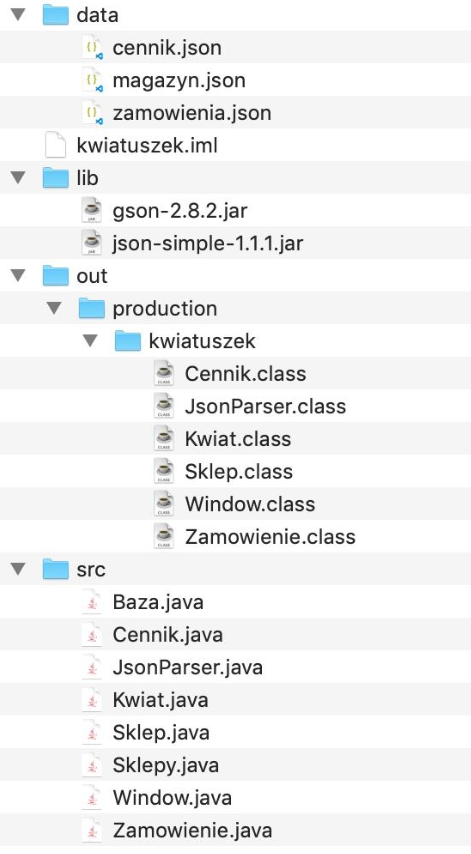
\includegraphics[scale=0.5]{struktura_plikow.PNG}
            \caption{Struktura plików projektu}
        \end{figure}
        
        \FloatBarrier
        
        
        \subsection{Algorytmy i biblioteki}
        \subsubsection{Biblioteka JSON.simple}
        Jest to biblioteka Javy, służąca do przetwarzania, odczytywania i zapisywania danych w plikach typu JSON. Dzięki niemu można przetwarzać obiekty typu JSONObject, JSONArray. Biblioteka zawiera także opcję parsowania, która bez wątpienia przyda się nam np. dla wczytywania zamówień lub magazaynów
        
        \subsubsection{Biblioteka Gson}
        Korzystając z biblioteki Gson można bardzo łatwo zapisywać obiekty Javy jako plik JSONowy. Bardzo ważne jest, żeby nazwy pól w klasie Javy były takie same jak nazwy obiektów w JSONie, ponieważ wykorzystuję ona nazwy atrybutów klasy żeby przepisać wartości w odpowiednie miejsce. Gson bardzo upraszcza pracę z odczytywaniem plików JSON, ponieważ sam przypisuje wszystkie potrzebne wartości według potrzebnych typów danych w konstruktorze tej klasy. Zamierzamy użyć tej biblioteki na pewno przy pisaniu klas "Kwiatuszek.Sklep" i "Kwiatuszek.Cennik", ułatwi nam to bardzo aktualizowanie stanów magazynów sklepów.
        
        \subsubsection{Algorytm wybierania sklepu}
        Jako iż zakładamy, że nasze sklepy znajdują się w niedużej odległości od siebie, nie musimy się przejmować rozdzielaniem zamówienia ze względu na odległość od klienta. Zatem jedynym dwoma parametrami wpływającym na wybranie danego sklepu jest jego stan magazynu jak i dostępne godziny kuriera. Dlatego postanowiliśmy zapisać wszystkie nasze sklepy w specjalnej kolejce FIFO, która nie wyrzuca elementów z kolejki, lecz zapisuje je z powrotem na końcu. W ten sposób będziemy iterować po każdym obiekcie klasy Kwiatuszek.Sklep. Każdy ze sklepów posiada metodę $"sprawdzSklep(zamowienie)"$ zwracającą \textbf{true}/\textbf{false} w zależności od tego czy podany sklep jest w stanie dane zamówienie zrealizować. Jeżeli operacja ta zwróci \textbf{true}, wtedy podany sklep wywołuje następna metodę $"przypiszZamowienie(zamowienie)"$, która zostaje obsługiwana wewnątrz iterowanego obiektu.
        
        
    \section{Etap 3}
        \subsection{Co nam się udało osiągnąć}
        
        \paragraph{Stworzenie Klasy $Kwiatuszek.Kwiat$ i $Kwiatuszek.Zamowienie$} Są to klasy służące do reprezentacji naszych zamówień. Nie było w nich dużo do zrobienia, zwykłe zdefiniowane atrybutów oraz zabezpieczeń.
        \paragraph{Stworzenie Klasy Kwiatuszek.Sklep} Jest to klasa dzięki, której tworzymy obiekty reprezentujące nasze sklepy. W skład tej klasy wchodzą między innymi metody:
        \begin{itemize}
            \item \textbf{sprawdzSklep(Kwiatuszek.Zamowienie)} - Metoda sprawdzająca czy podane zamówienie jest możliwe do zrealizowania dla danego obiektu
            \item \textbf{przypiszZamowienie(Kwiatuszek.Zamowienie)} - Metoda, która realizuje podane zamówienie, zmieniając stan magazynu oraz rezerwując godzinę dostawy obiektu.
        \end{itemize}
        \paragraph{Stworzenie Klasy Kwiatuszek.Baza} Jest to nasza główna klasa reprezentująca cały system poczty kwiatowej. Znajdują się w niej instancje wszystkich zamówień jak i sklepów. To właśnie w niej rozprowadzane są zamówienia do konkretnych sklepów. W skład tej klasy wchodzą między innymi metody:
        \begin{itemize}
            \item \textbf{wczytajZamowienia(PATH)} - Metodą sczytująca dane z plików JSON, na podstawie których tworzymy obiekty klasy $Zamówienie$
            \item \textbf{wczytajSklepy(PATH)} - Metodą sczytująca dane z plików JSON, na podstawie których tworzymy obiekty klasy $Kwiatuszek.Sklep$
        \end{itemize}
        
        
        \subsection{Napotkane problemy}\begin{itemize}
            \item \textbf{Praca z plikami JSON} - Pierwszym dużym problemem było znalezienie narzędzi za pomocą których moglibyśmy odczytać plik JSON (ponieważ tworzenie własnych metod byłoby bardzo długie oraz nieopłacalne). Na początku próbowaliśmy korzystać z biblioteki $json-simple$, niestety okazało się, że biblioteka ta posiada problem w zapisywaniu zagnieżdżonych plików. Dalej po długim wyszukiwaniu znaleźliśmy bibliotekę $GSON$, z którą wczytywanie (jak potem i zapisywanie nowych danych) poszło stosunkowo szybko i przyjemnie. 
            \item \textbf{Spójność kodu} - Oczywistym problemem, który pojawił się w niewielkim stopniu był bałagan w naszym repozytorium. Nie ustaliliśmy podstawowych zasad co do etyki kodu, za co musieliśmy później ponieść konsekwencje.
            \item \textbf{Wykorzystywanie narzędzia git} - Do tej pory pracowaliśmy wszyscy na jednym, głównym branchu $master$.W konsekwencji pojawiły się problemy z zaległymi commitami. Nie było to optymalne i bezpieczne rozwiązanie, szczególnie, że mamy do dyspozycji potężne narzędzie systemu git, które otwiera nam drogę na nowe możliwości.
        \end{itemize}
        
        \subsection{Pomysły na dalsze etapy}
        Aktualnie staramy się dokończyć wszystkie cele, które zostały ustalone na samym początku projektu. Jednakże pojawiły się też różne pomysły mające na celu refaktoryzację naszego kodu. Główną rzeczą jaka nam została jest optymalne rozdzielanie zamówień pomiędzy sklepami oraz stworzenie klasy Kwiatuszek.Log, mającej za zadanie notowanie działań w systemie. Mamy również plan rozbudować recepturę naszych zamówień tak aby posiadały one parametr mówiący o lokalizacji złożenia zamówienia. Chcemy aby ten czynnik wpływał na rozdzielenie naszych zasobów pomiędzy sklepami.
    
    \section{Etap 4}
        \subsection{Co nam się udało osiągnąć}
        \subsubsection{Poprawki}
        W trakcie tego etapu przyjrzeliśmy się naszemu dotychczasowemu kodowi. Omówiliśmy, jakie poprawki możemy wykonać, aby kod był bardziej przejrzysty i czytelny dla wszystkich członków grupy. Wśród zmienionych elementów można wymienić m.in.: użycie bardziej czytelnej pętli for, zamieszczanie elementów typu zmienne, gettery, override w konkretnych miejscach w pliku, używanie jednolinijowych kodów oraz inne stylistyczne poprawki.W związku z tym,zmieniliśmy nieco kod klasy Kwiatuszek.Sklep oraz pozmienialiśmy kilka metod (naprawiliśmy kilka błędów w przydzielaniu zamówień oraz w sprawdzaniu sklepów). Została również utworzona nowa metoda w klasie Kwiatuszek.Baza, która wczytuje zamówienie, wyznacza kwotę do zapłaty zgodnie z danymi w cenniku a następnie ją zwraca. Zdecydowaliśmy, że zaczniemy komentować nasz kod (poza oczywistymi zmiennymi i zrozumiałymi metodami) by osoba trzecia była w stanie zrozumieć i przeanalizować kod. Uzgodniliśmy również typy danych w programie, żeby dane były wygodne do wykorzystania przez inne metody w innych klasach.
        \subsubsection{Utworzenie klasy Kwiatuszek.Log}
        Utworzyliśmy pierwszą, podstawową wersję klasy Kwiatuszek.Log, której zadaniem będzie zapisywanie do pliku log procesów, jakie zachodzą w naszym systemie. Utworzona klasa to wersja bardzo podstawowa, wymagająca poprawek do prawidłowego funkcjonowania.
        \subsubsection{Przypisywanie zamówień}
        Kolejnym utworzonym elementem było stworzenie metod, które służą do przypisywania zamówień do sklepów i obliczania ich ceny. Metoda do przypisywania zamówienia nie jest jeszcze gotowa, ponieważ występują problemy.
        \subsection{Napotkane problemy}
        Pierwszym problemem jest poprawne przypisywanie zamówień. Występuje tutaj problem z biblioteką GSON, która po wczytaniu danych usuwa wszystkie dane z pliku.
        
        
        Kolejnym problemem napotkanym w tym etapie była klasa Kwiatuszek.Log. Nie działa ona jeszcze zgodnie z naszymi oczekiwaniami i nie spełnia prawidłowo swojej funkcji.
        \subsection{Pomysły na dalsze etapy}
        Naszym celem na kolejny etap jest ukończenie klasy Kwiatuszek.Log, tak aby wpisywała konkretne parametry do pliku (np. co konkretnie zostało wczytane w zamówieniu, do jakiego sklepu zostało przydzielone itd.). Planujemy udoskonalić metodę z obsługą pliku json przez bibliotekę GSON, tak aby dane nie były usuwane. Będziemy także testować nasz program i reagować na niezauważone do tej pory błędy.
    
    \clearpage
    
    \section{Etap 5}
        \subsection{Co nam się udało osiągnąć}
        W tym etapie zmieniliśmy trochę koncepcję naszego projektu i postanowiliśmy dodać specjalne Kwiatuszek.Kwiatuszek.GUII dla użytkownika. Poprzednim naszym zamysłem było składowanie listy zamówień w specjalnym pliku jsonowym, który po uruchomieniu programu przypisałby je odpowiednim sklepom. Jednakże w ostatnim czasie na zajęciach z programowania nauczyliśmy się tworzyć proste interfejsy graficzne. Wpadliśmy zatem na pomysł zaimplementowania naszych nowych umiejętności do projektu. Nie chcieliśmy jednak bezsensownie pisać całego kodu "Kwiatuszka" od nowa, więc postanowiliśmy, że interfejs Kwiatuszek.Kwiatuszek.GUII będzie służył jako swego rodzaju kreator listy zamówień, a konkretnie naszego pliku jsonowego. W ten sposób nie będziemy musieli tworzyć całego systemu Bazy od nowa i możemy jedynie "doczepić" samą aplikacje.
        
        
        \begin{figure}[hbt]
                \centering
                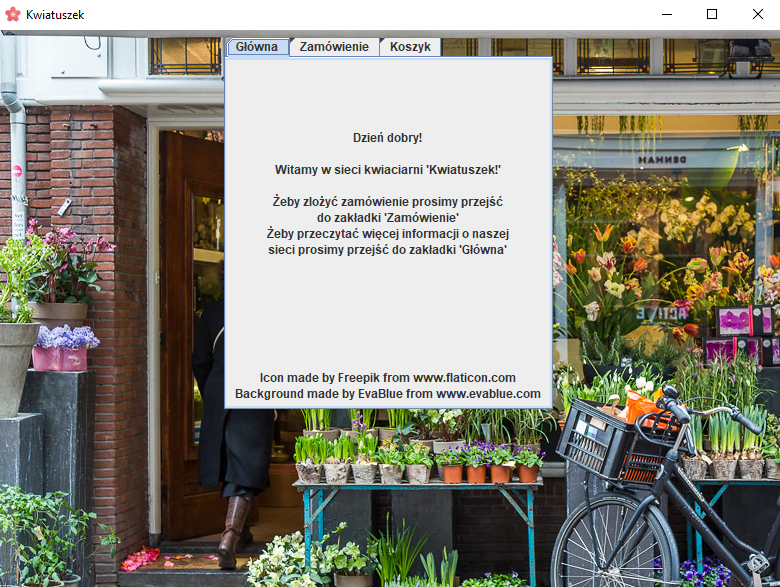
\includegraphics[scale=0.6]{prototyp_kwiatuszka.PNG}
                \caption{Dotychczasowy prototyp naszego Kwiatuszek.Kwiatuszek.GUII}
        \end{figure}
        
        Podzieliliśmy nasz program na 3 różne zakładki:
        \begin{itemize}
            \item Główna: \newline
            Zakładka startowa, na której znajdują się ogólne informacje jak i instrukcja dotycząca korzystania z naszej aplikacji.
            \item Zamówienie \newline
            Służy ona do dodawania kwiatów do naszego koszyka.
            \item Koszyk\newline
            Wyświetla obecny stan koszyka oraz można z jej poziomu złożyć zamówienie. 
        \end{itemize}


        \subsection{Napotkane problemy}\begin{itemize}
        
            \item \textbf{Brak spójnej wizji projektu} -
            Podczas tworzenia naszego Kwiatuszek.Kwiatuszek.GUII mieliśmy problem związany z różnymi wersjami interfejsu, który ma powstać. W pierwotnym zamyśle ustaliliśmy, że będzie to graficzna wersja przyjmowania różnych zamówień do bazy. Jednak w trakcie pracy część zespołu zrozumiała, że ma być to zwykła aplikacja, którą będzie obsługiwał użytkownik. Problem jednak został szybko rozwiązany poprzez spotkanie się i omówienie wspólnej koncepcji.
            \item \textbf{Problemy z Gitem}
            Także w tym etapie mieliśmy problem z Gitem. W dalszym ciągu pracowaliśmy na jednym branchu. Ponieważ wszyscy pracowali na tych samych plikach, skutkowało to w pojawianiu się konfliktów. Dzięki temu jednak wszyscy z zespołu dowiedzieli się jak należy czytać komunikaty związane z konfliktem (np. HEAD >>>).
        \end{itemize}
        \subsection{Podsumowanie}
        Na ostatnie tygodnie realizacji projektu planujemy dokończyć nasze Kwiatuszek.Kwiatuszek.GUII. Dopracujemy to co już zostało w nim stworzone, oraz dokończymy ostatnią zakładkę "Koszyk". Następnie dokonamy testów na naszych programach i zakończymy tym pracę nad kodem naszej sieci kwiaciarni.
\end{document}